\chapter[疑问句,否定句]{疑问句,否定句}
%\chapter[短标题显示在页面]{长标题显示在目录}

  



\emoji{l_diina}
这是我前几天在公园散步时看见的花.

紫苑,这是樱花吗?
\begin{figure}[H]
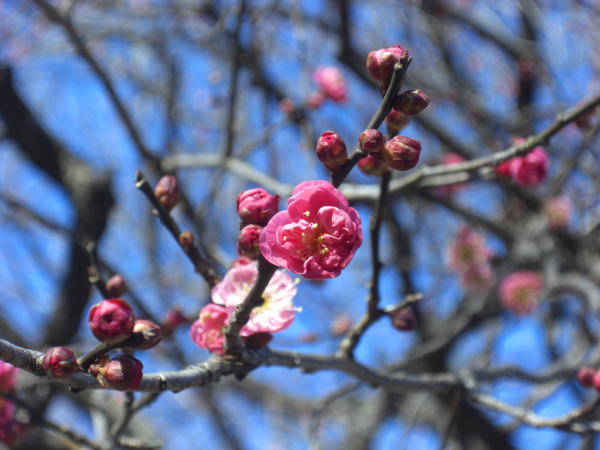
\includegraphics[width=0.7\textwidth]{ARKA/ping.jpg}
\end{figure}

\emoji{x_lo}
额,这是梅花,不是樱花哟

呐,在Arka里怎么说"这是梅花."?

\emoji{l_asex_kal}
"这是梅花"应该说"tu et ping"。"tu et"就是上次讲过的

"这是樱花"也差不多,说"tu et seron"。

"这是樱花吗"就在句子最后加上mia."tu et seron mia?"

不过很多场合我们不特意加"mia",只是在句子后面加一个问号.


\emoji{x_pil}
疑问的时候语调要上扬一些呢.
相比于英语的"Do you...?"Arka要简单呢。跟汉语在句末加"吗"比较像.


\emoji{l_sena}
另一方面,"这不是樱花"应该说"tu de seron".
de一个词就表示系动词的否定,像是"isn't"一样.
顺便一说,女生不用"de",而用"te".


\emoji{x_niit}
那么我其实应该说"tu te seron"吗.

%ともあれ、「~でない」はdeね。「~DEない」と覚えようw ------翻译不过来的梗
另外,"不写"应该怎么说呢?


\emoji{l_xanxa}
be动词以外嘛,就在动词前面放副词"en".

axt是"写"、那么"en axt"就是"不写".


\emoji{x_demo}
哦......"紫苑不写Arka"就是"xion en axt arka"吧。

让我总结一下:

\textbf{
疑问句:只是在句尾加"mia"\\
否定句:be换成de,另外就是在动词前面加"en".
}

\emoji{l_deyu}
最后来做个小测试吧.

试着写下"这是猫吗?","这不是猫,是狗.","紫苑会写Arka吗?"这三个句子
答案就在下回的开头.atte!(加油!)




%``([a-z]+)''
%``$1''


